\documentclass[12pt]{article}
\usepackage{bera}
\usepackage{beramono}
\usepackage{enumerate}
\usepackage[letterpaper]{geometry}
\setlength{\footskip}{53pt}
\usepackage{graphicx}
\usepackage{float}
\title{\vspace{4cm}\begin{Huge}
InstiOverflow\\[0.2cm]
\end{Huge}
\begin{LARGE}
Software Lab
\end{LARGE}
}
\author{\begin{Large}
 INDIAN INSTITUTE OF TECHNOLOGY, BOMBAY
 \end{Large}}
\date{
\begin{Large}
				\textit{$
				27^{th} November,2020$}
			\end{Large}}

\begin{document}
	
 	\begin{titlepage}
 		
 		\maketitle
 		\begin{center}
 		\begin{Large}
				Ashwani Kumar Jha\\[0.2cm]
		\end{Large}
		\begin{large}
		20305R001
		\end{large}
		\end{center}
		
		\begin{center}
 		\begin{Large}
				Pranjal Saini\\[0.2cm]
		\end{Large}
		\begin{large}
		203050014
		\end{large}
		\end{center}
		
		\begin{center}
 		\begin{Large}
				Shubham Nemani\\[0.2cm]
		\end{Large}
		\begin{large}
		203050011
		\end{large}
		\end{center}
		
		\begin{center}
 		\begin{Large}
				Harsh Peswani\\[0.2cm]
		\end{Large}
		\begin{large}
			203050043
		\end{large}
		\end{center}
		
	
				
 		\thispagestyle{empty}
	\end{titlepage}
	

\tableofcontents
\pagebreak
\section{Introduction}

InstiOverflow is a webapp similar to stackoverflow exclusively for IITB. In this anybody
from IITB can post question by selecting appropriate Subject like Machine Learning, Software Lab,
Systems etc and others can answer it.\\\\
In this user have to select subject from the list provided in dashboard, and then he/she will see Questions, Tags of particular question, Number of Answers in that particular question,Number of Comments and Time of when it was posted.He/She will also see Add Question Button Using this he/she can post questions of that particular subject.\\\\
Questions/Answers/Comments can be deleted only by the person who posted it.Others cannot delete the questions posted by someone else.This project will facilitate peer to peer discussion which is lacking in this online semester.



\section{Motivation}
We have observed that the most lacking thing in this online semester is peer to peer discussion.Though there exists Moodle discussion forum, but there is no peer to peer discussion going on there.The person who asked the question expects TAs or the Professor to answer. So its not facilitating peer to peer discussions.Another solution was to use whatsapp but it has a huge drawback that after certain period of time, the context of discussion changes to something else.\\\\
Peer to Peer discussion is important because it helps to understand the concepts better and also helps us to see the problem with multiple dimensions.\\\\
Due to this online semester, we have faced that there is lack of discussion
among peers. Our project aims at creating a global discussion forum in which
students throughout the institute can participate and this will motivate
discussion between peers

\section{Dependencies}
\begin{large}
	Back-end
\end{large}

\begin{itemize}
	\item handling server requests: `Node.js with Express.js Framework`
	\item Database: `MySQL`
 \item API tested using: `POSTMAN`

\end{itemize} 

\begin{large}
	\hspace{-0.7cm} Front-end
\end{large}

\begin{itemize}
\item Front-end Framework: `React.js (with Redux and react-router)`
\item Styling: `SASS` and `BOOTSTRAP`

\end{itemize} 


\section{Using InstiOverflow}
To use Instioverflow you need to install the following dependencies using following commands in ubuntu\\
\begin{itemize}


\item Install node and npm \dots{}
\begin{itemize}
	\item  sudo apt install nodejs
	\item  node -v   (check version of node)
	\item sudo apt install npm
	\item npm -v   (check version of npm)

\end{itemize}

\item Install mysql \dots{}
\begin{itemize}
	\item  sudo apt update
	\item  sudo apt install mysql-server
\end{itemize}

\item setup mysql user and server \dots{}
\begin{itemize}
	\item  sudo mysql
	\item  mysql>ALTER USER 'root@localhost' IDENTIFIED WITH mysql\_ native\_ password  BY mysql@123; (change password of root mysql@123 in this case)
	\item mysql>SET GLOBAL sql\_ mode=(SELECT REPLACE(@@sql\_ mode,'ONLY\_ FULL\_ GROUP\_ BY',''));
	\item mysql>flush privileges;
	\item mysql>exit
	\item mysql -u root -p

\end{itemize}
\item Run these commands then - 
\begin{itemize}


	\item npm install (Run this command in UI , API and instiOverflow folder)

\end{itemize}
	
	\item Run `instiOverflow.sql` file in the mysql client



\begin{itemize}
\item mysql -u root -p  < instiOverflow.sql   (user-root)
\end{itemize}

\item  Start the servers
\begin{itemize}
\item  npm run instioverflow 
\end{itemize}



\end{itemize}

\subsection{SignUp}
Enter username and password to signup\\


\begin{figure}[H]
\begin{center}
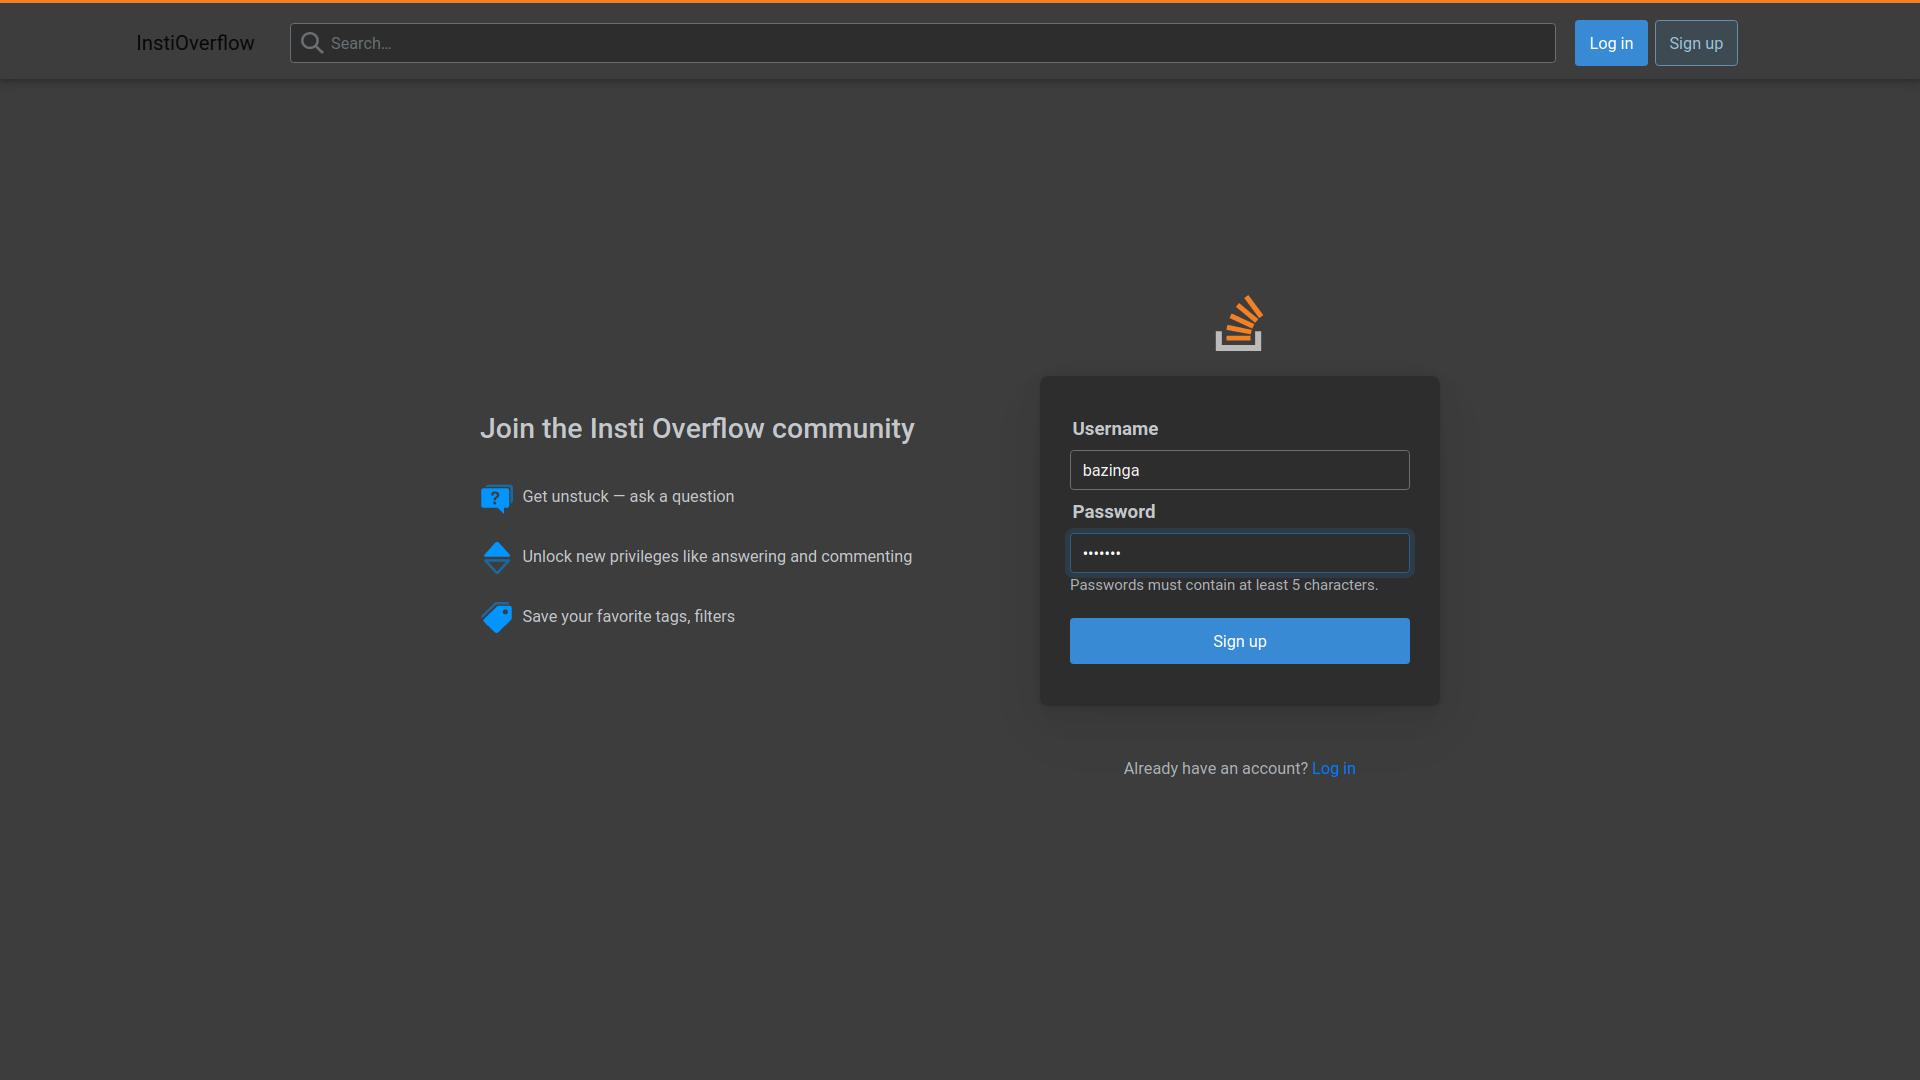
\includegraphics[width=0.75\columnwidth]{Signup}
\end{center}
\end{figure}

\subsection{SignIn}
Enter username and password to signin\\


\begin{figure}[H]
\begin{center}
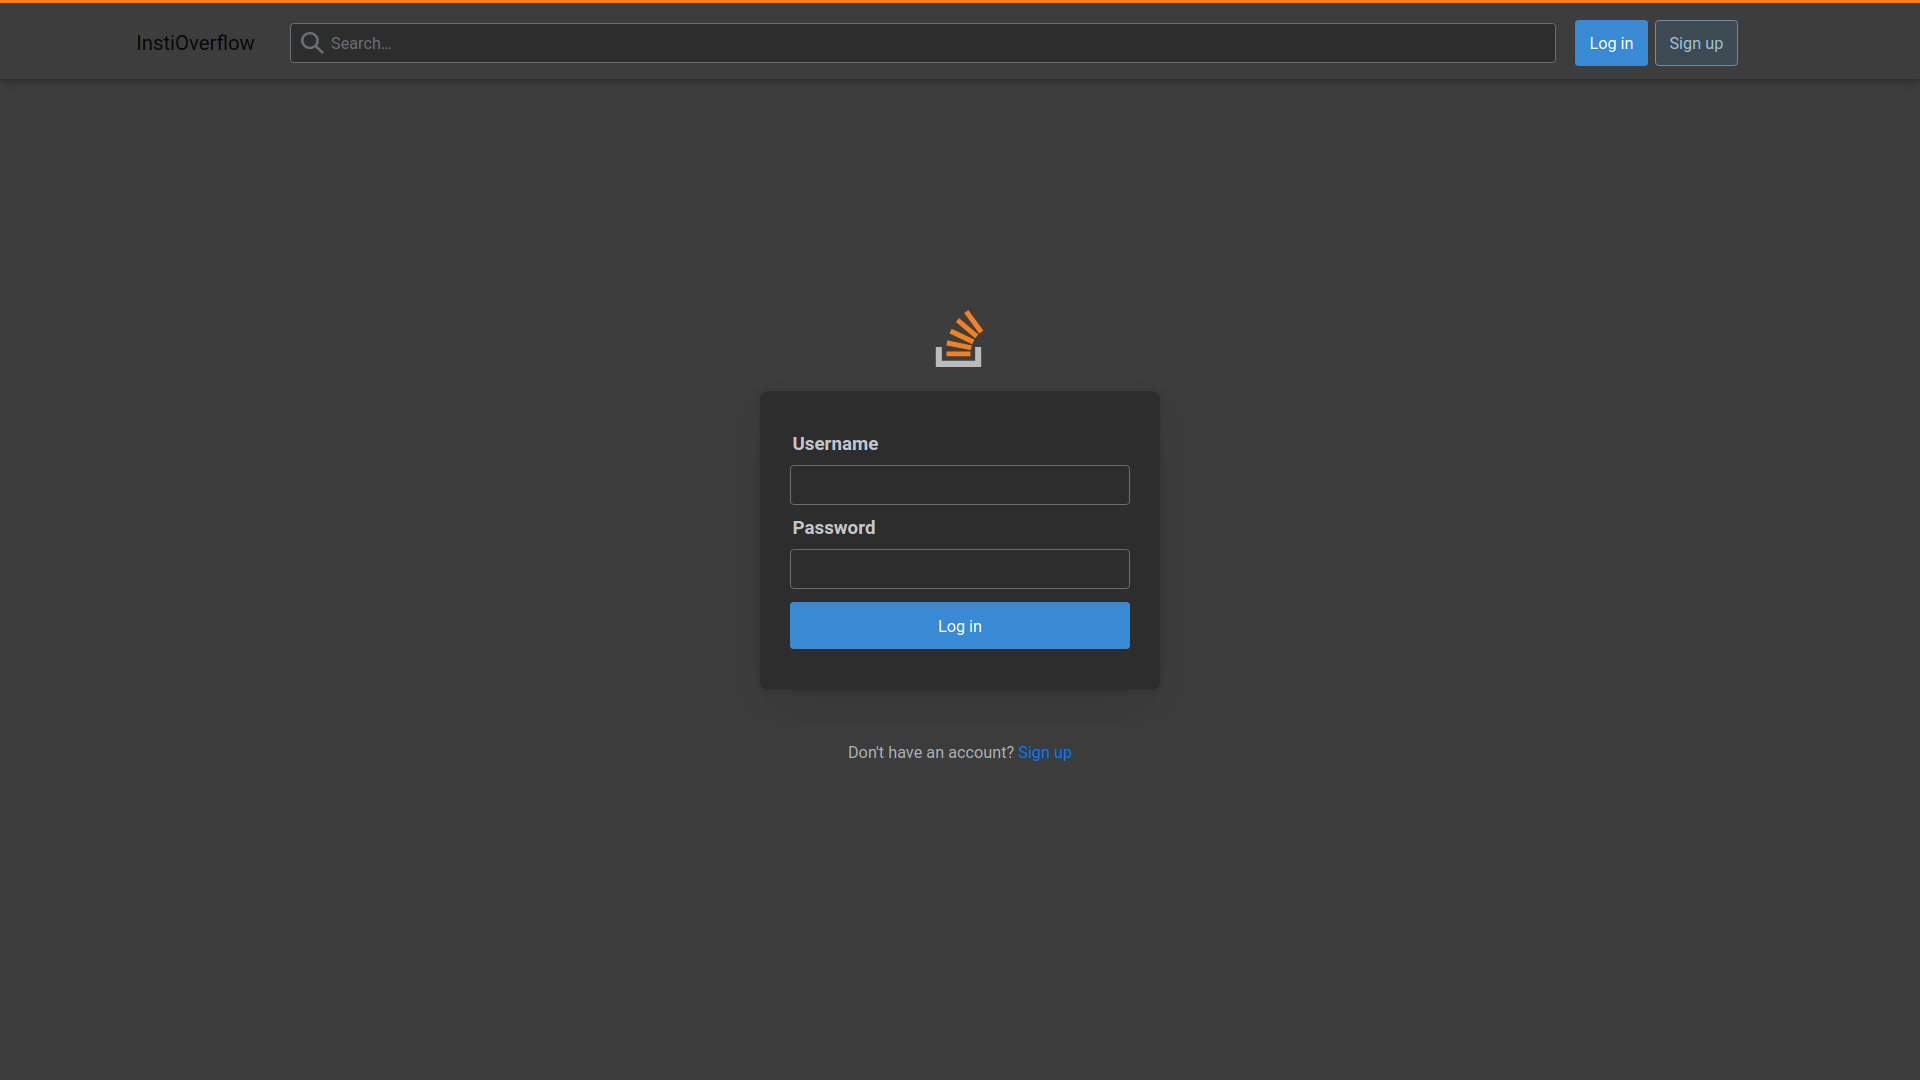
\includegraphics[width=0.75\columnwidth]{Login}
\end{center}
\end{figure}

\subsection{Dashboard}
Click on any subject\\


\begin{figure}[H]
\begin{center}
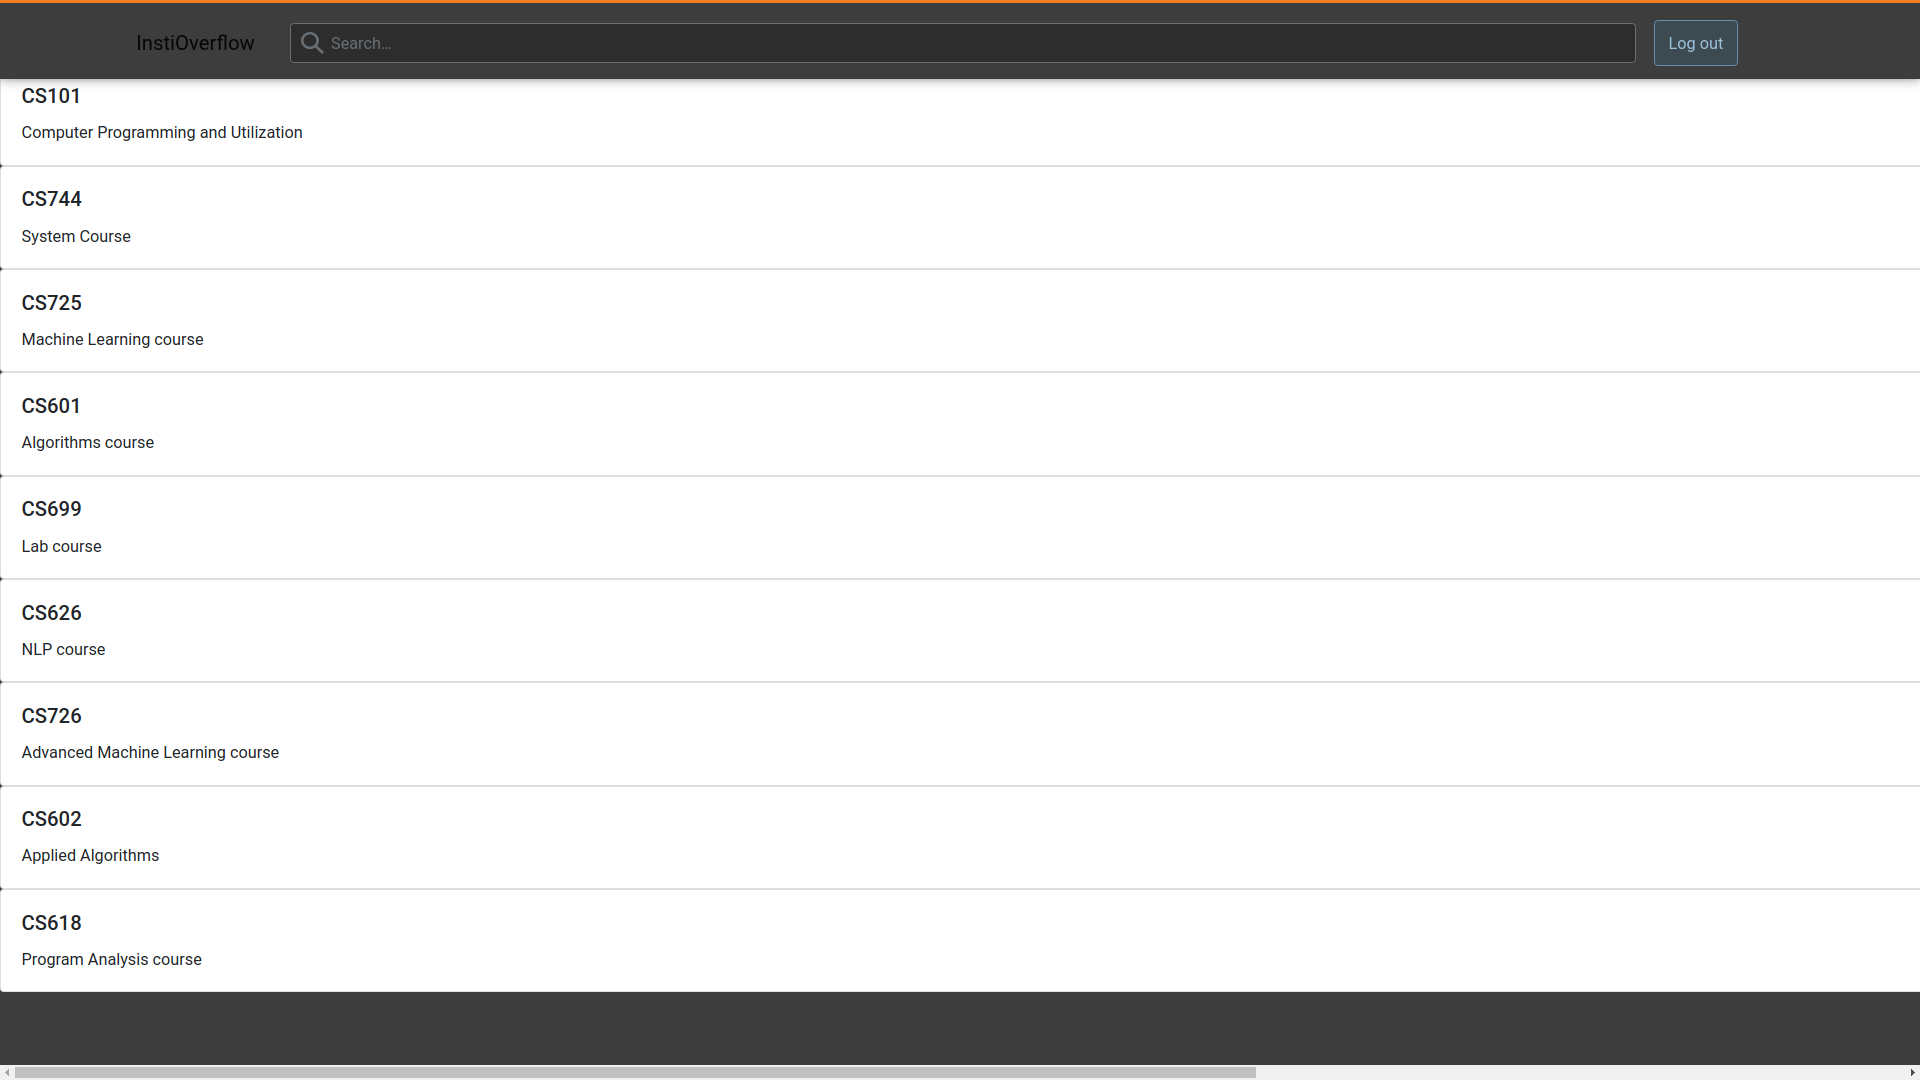
\includegraphics[width=0.75\columnwidth]{Dashboard}
\end{center}
\end{figure}

\subsection{View Questions}
Select Any Question\\


\begin{figure}[H]
\begin{center}
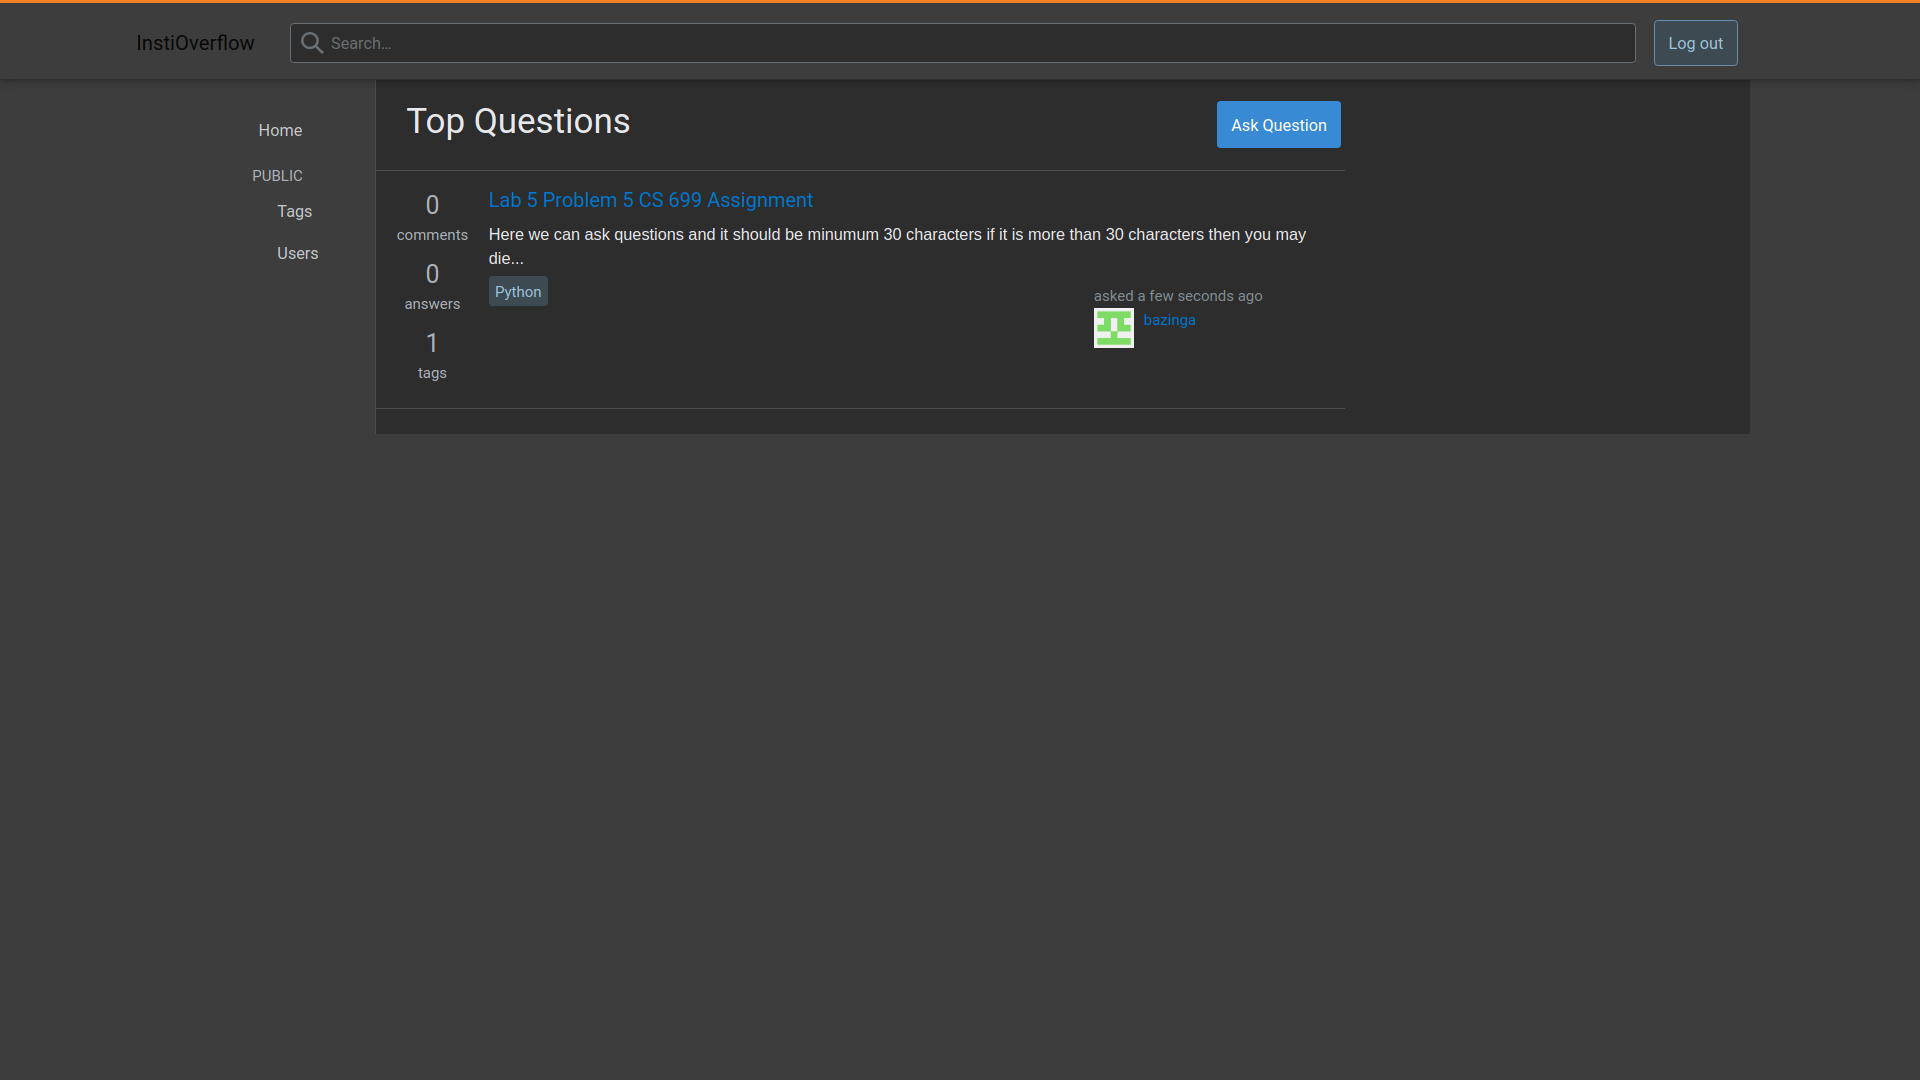
\includegraphics[width=0.75\columnwidth]{Viewsubject}
\end{center}
\end{figure}

\subsection{View Particular Question}



\begin{figure}[H]
\begin{center}
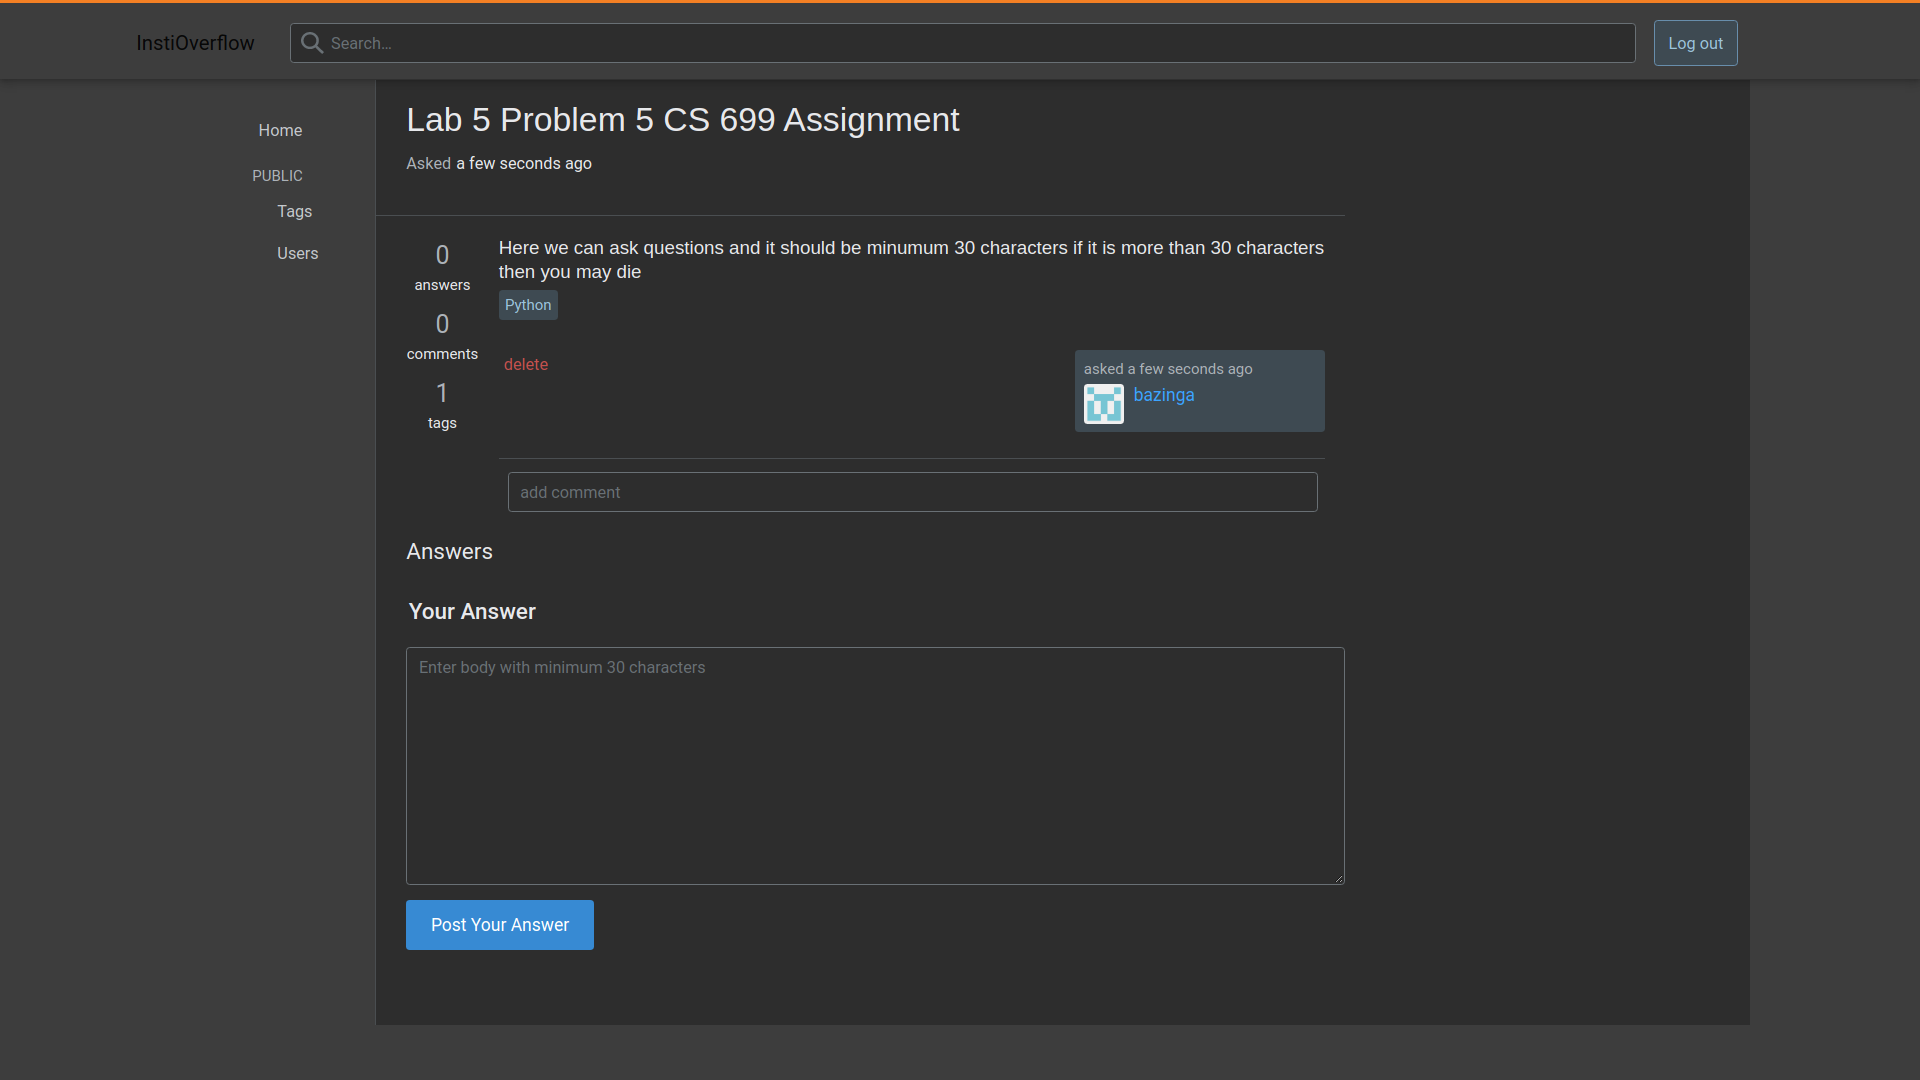
\includegraphics[width=0.75\columnwidth]{Viewquestion}
\end{center}
\end{figure}


\subsection{Answer}
Enter Your Answer\\


\begin{figure}[H]
\begin{center}

\includegraphics[width=0.75\columnwidth]{Answer}
\end{center}
\end{figure}

\subsection{Comment}
You can also comment on question or answer\\


\begin{figure}[H]
\begin{center}
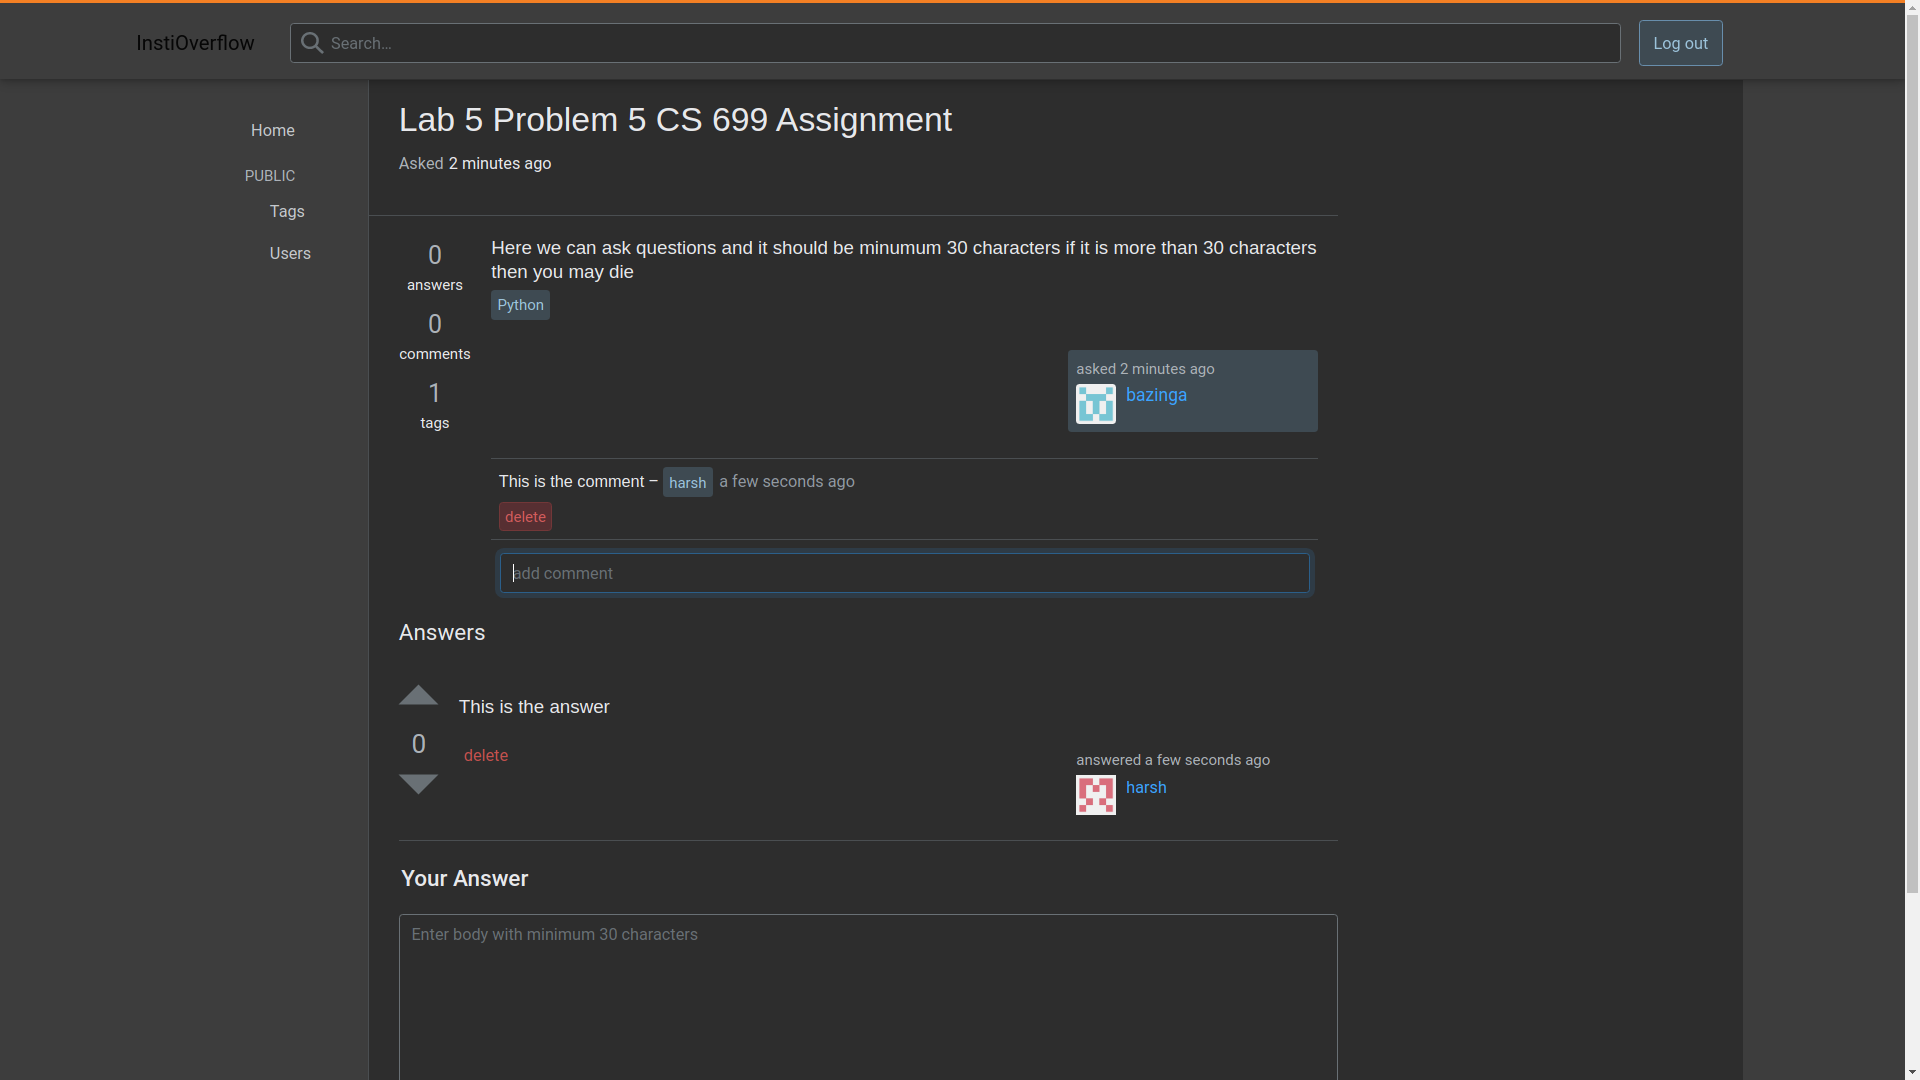
\includegraphics[width=0.75\columnwidth]{Comment}
\end{center}
\end{figure}

\subsection{Add Question}
You can Add Question by filling all the required fields\\


\begin{figure}[H]
\begin{center}
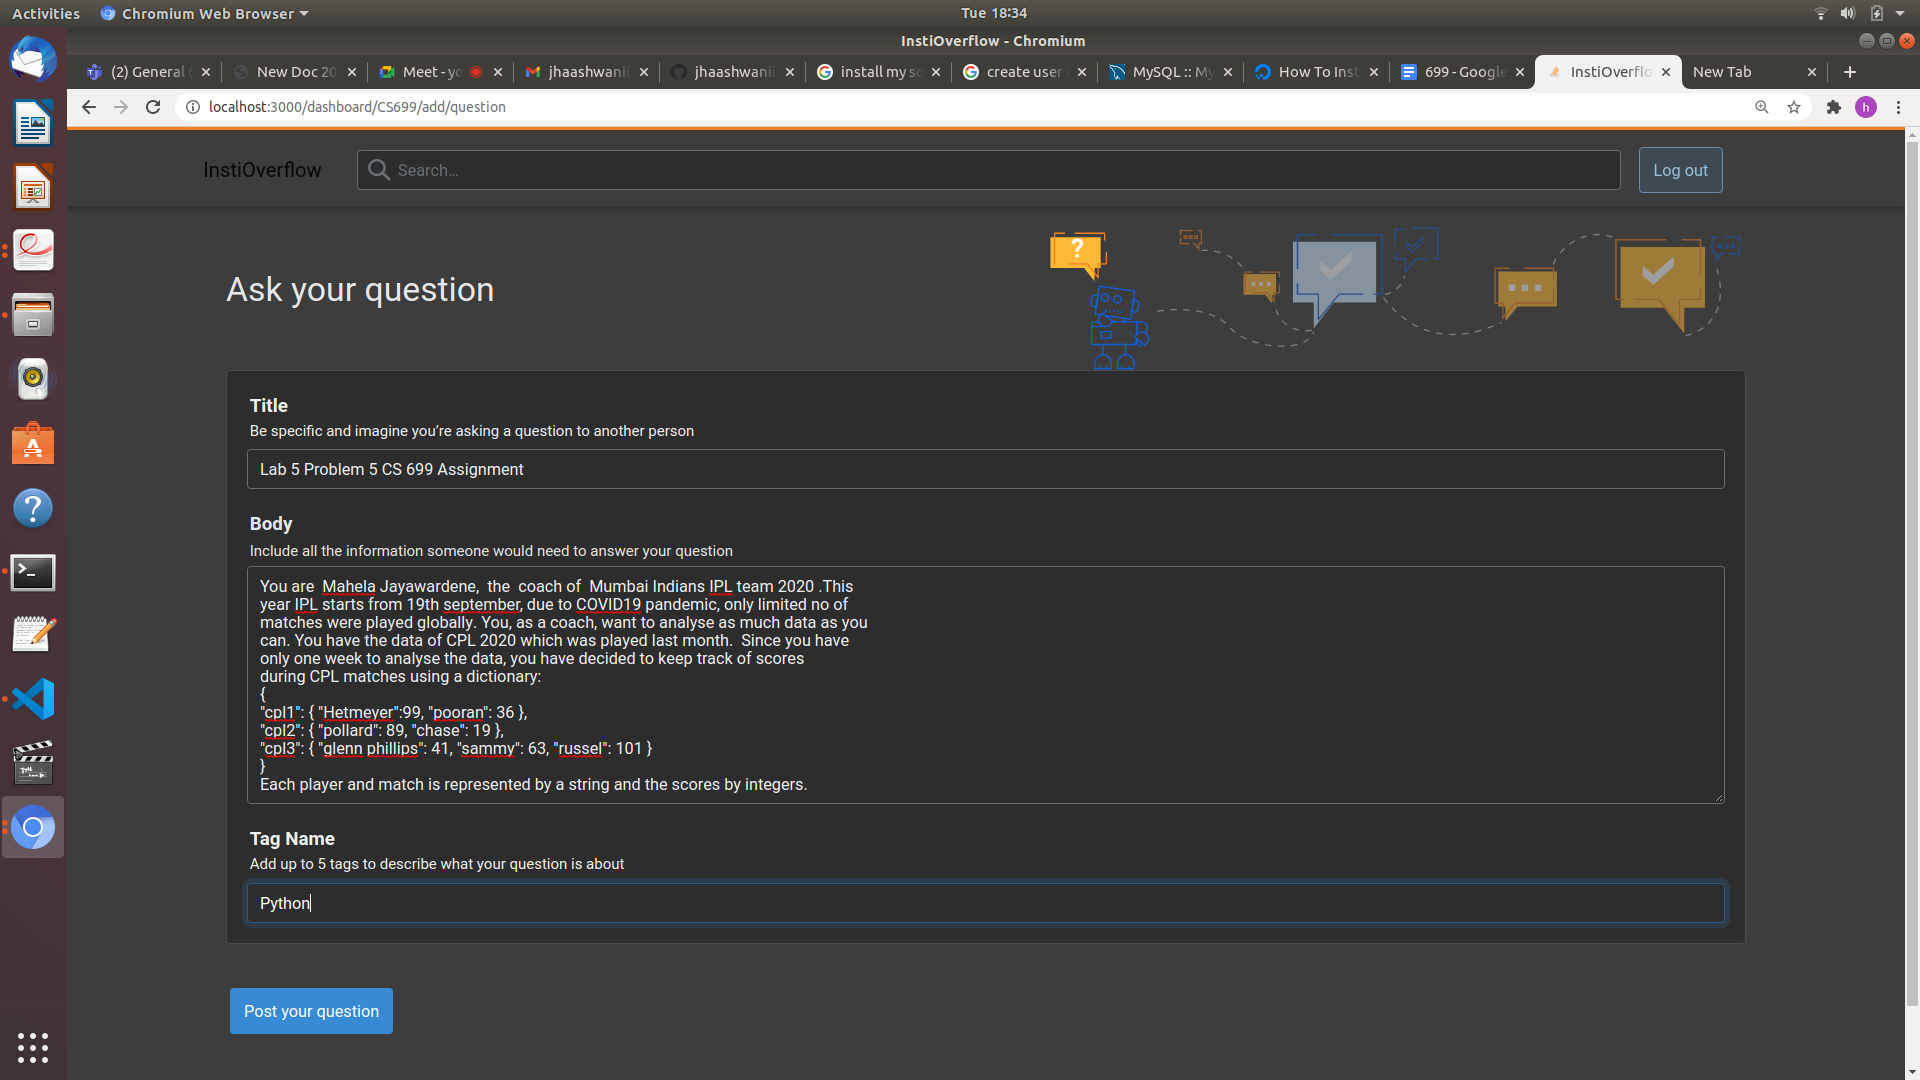
\includegraphics[width=0.75\columnwidth]{Addquestion}
\end{center}
\end{figure}

\subsection{View Tags}

\begin{figure}[H]
\begin{center}
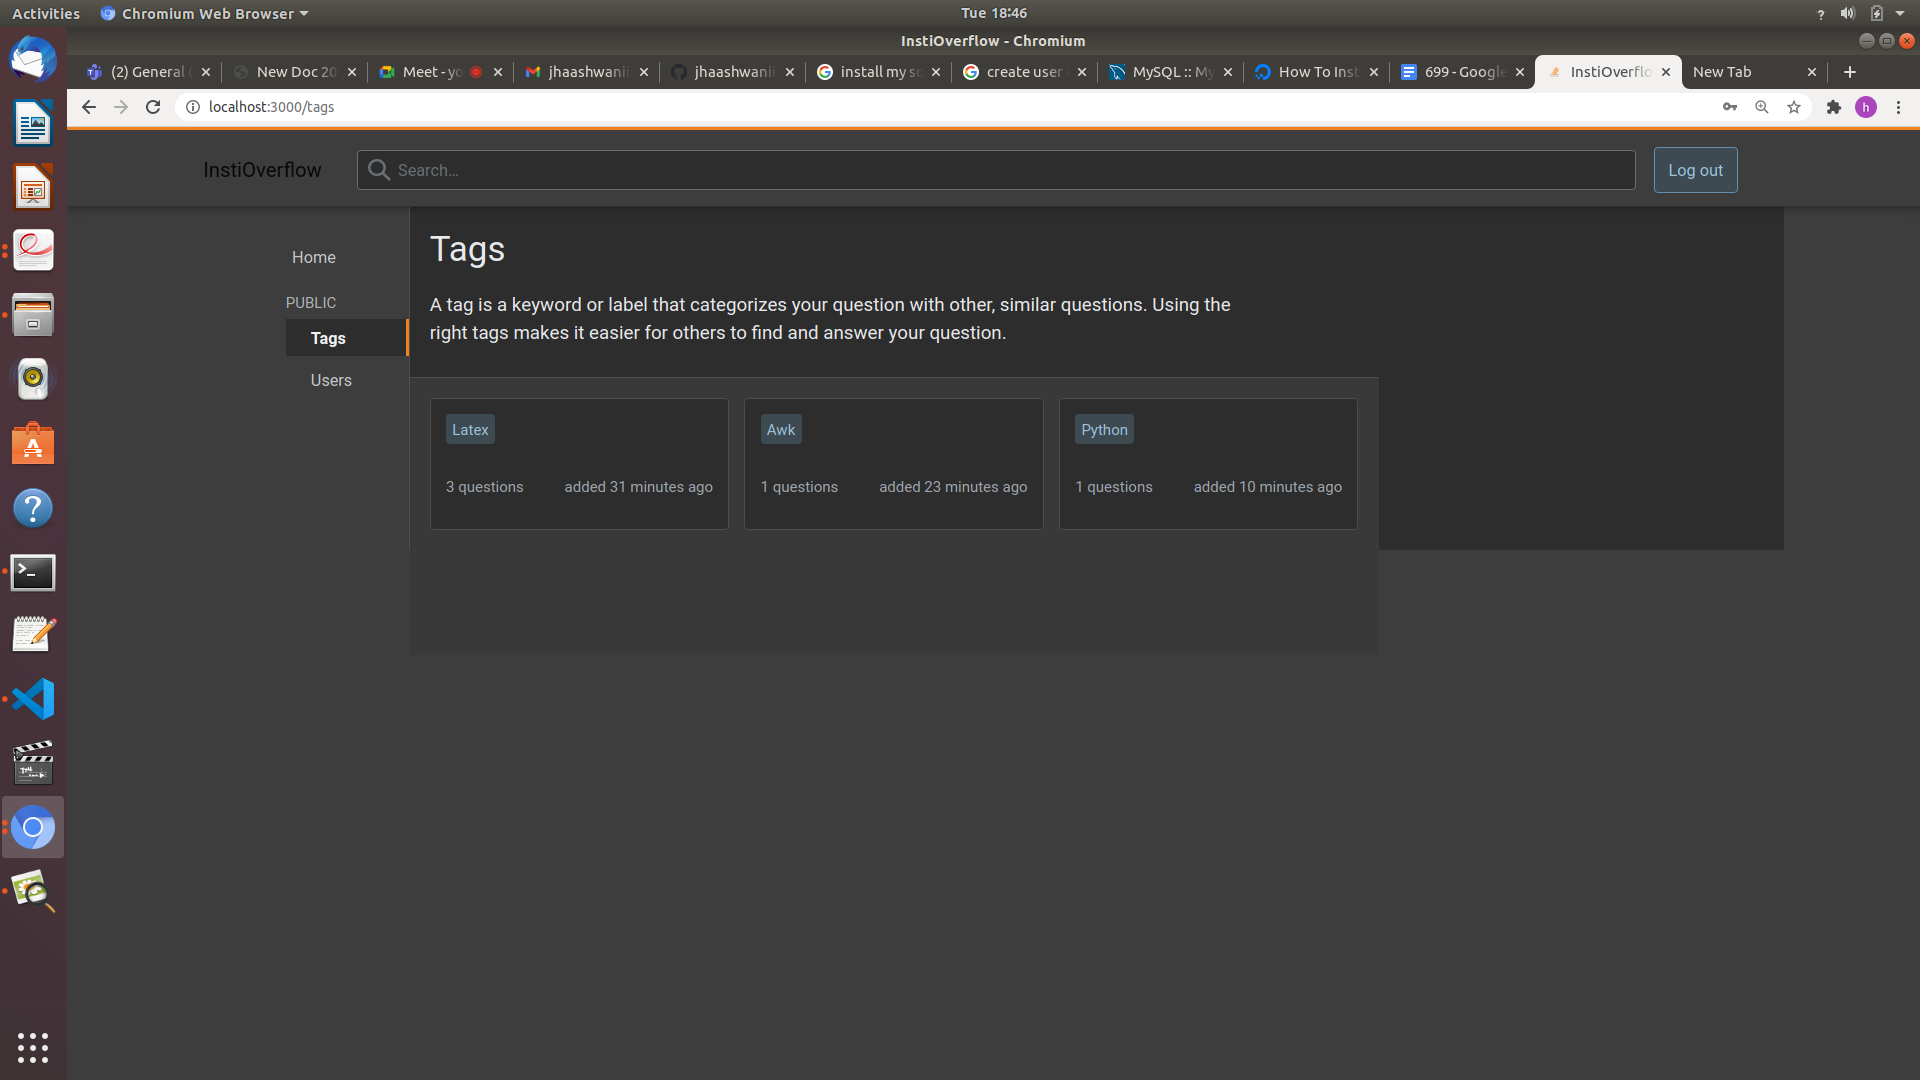
\includegraphics[width=0.75\columnwidth]{Tags}
\end{center}
\end{figure}

\subsection{View All Users}



\begin{figure}[H]
\begin{center}
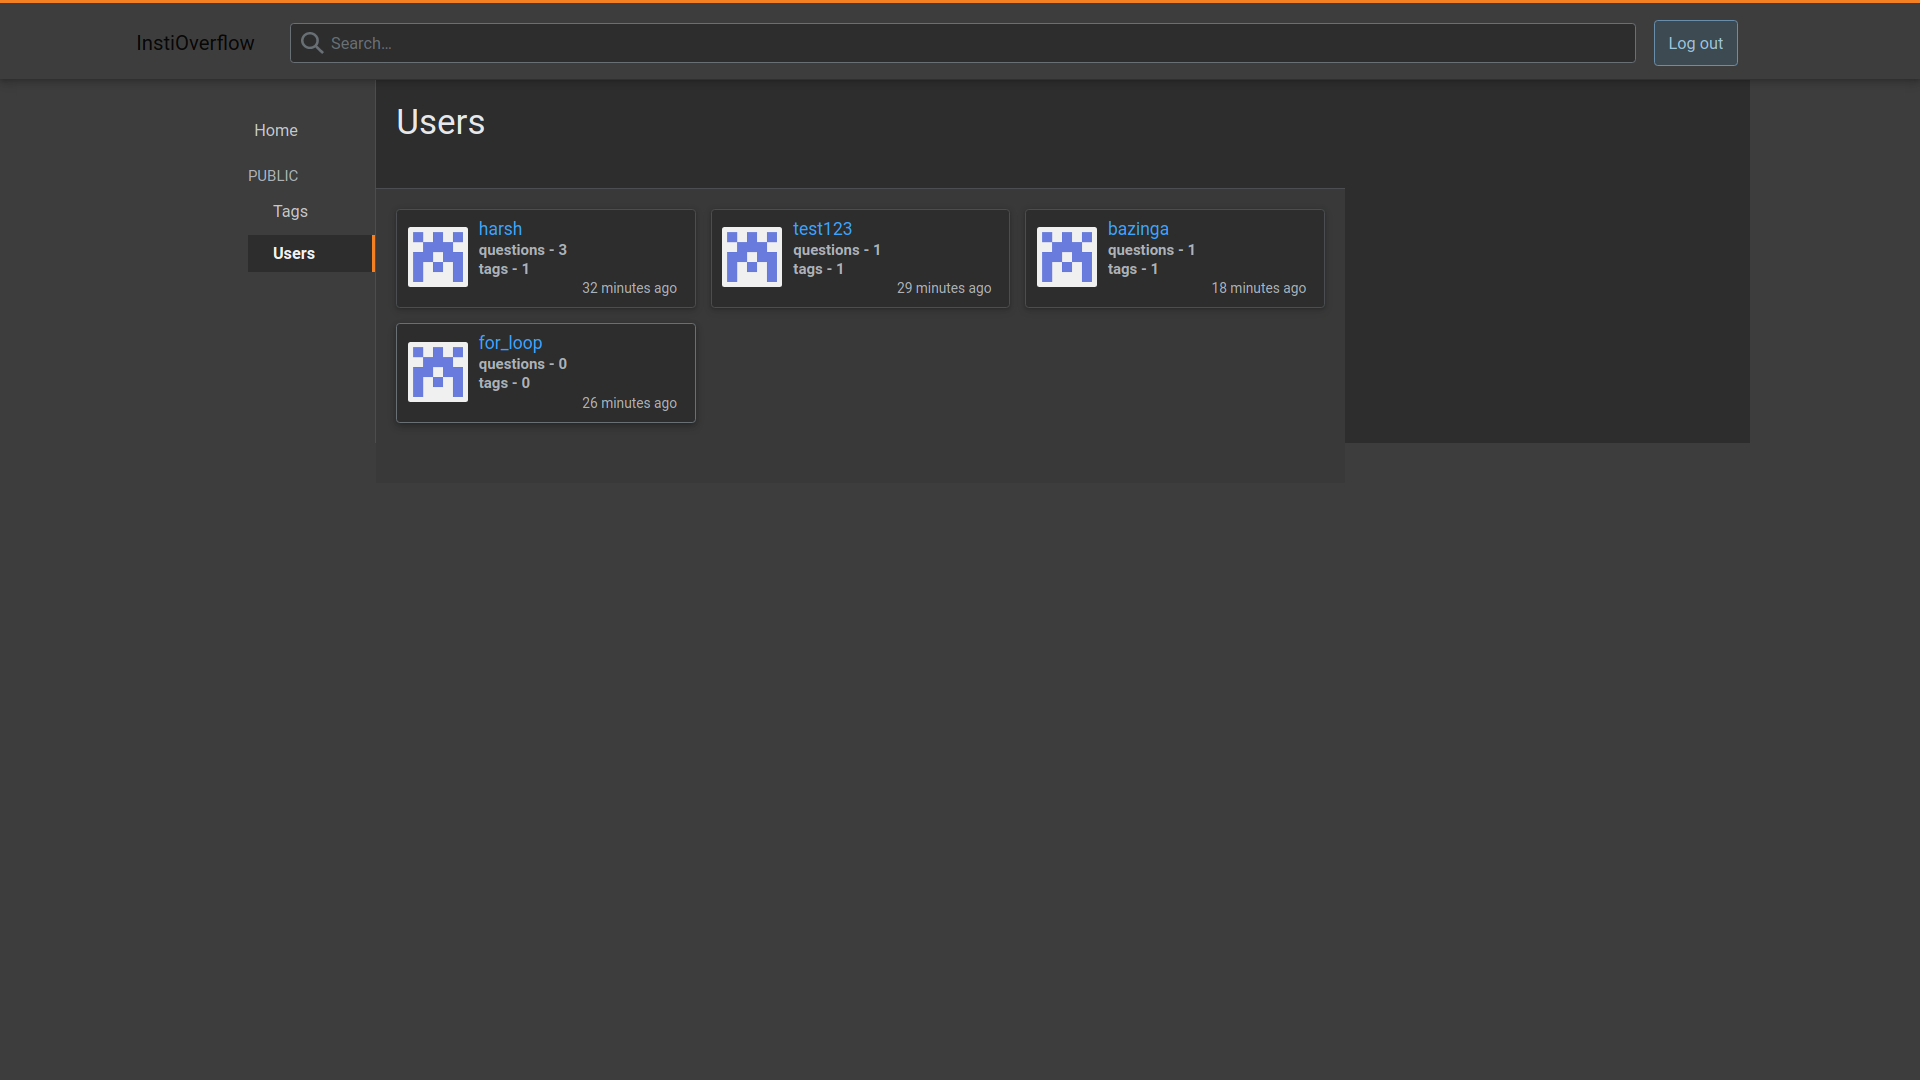
\includegraphics[width=0.75\columnwidth]{Users}
\end{center}
\end{figure}

\subsection{View Profile}


\begin{figure}[H]
\begin{center}
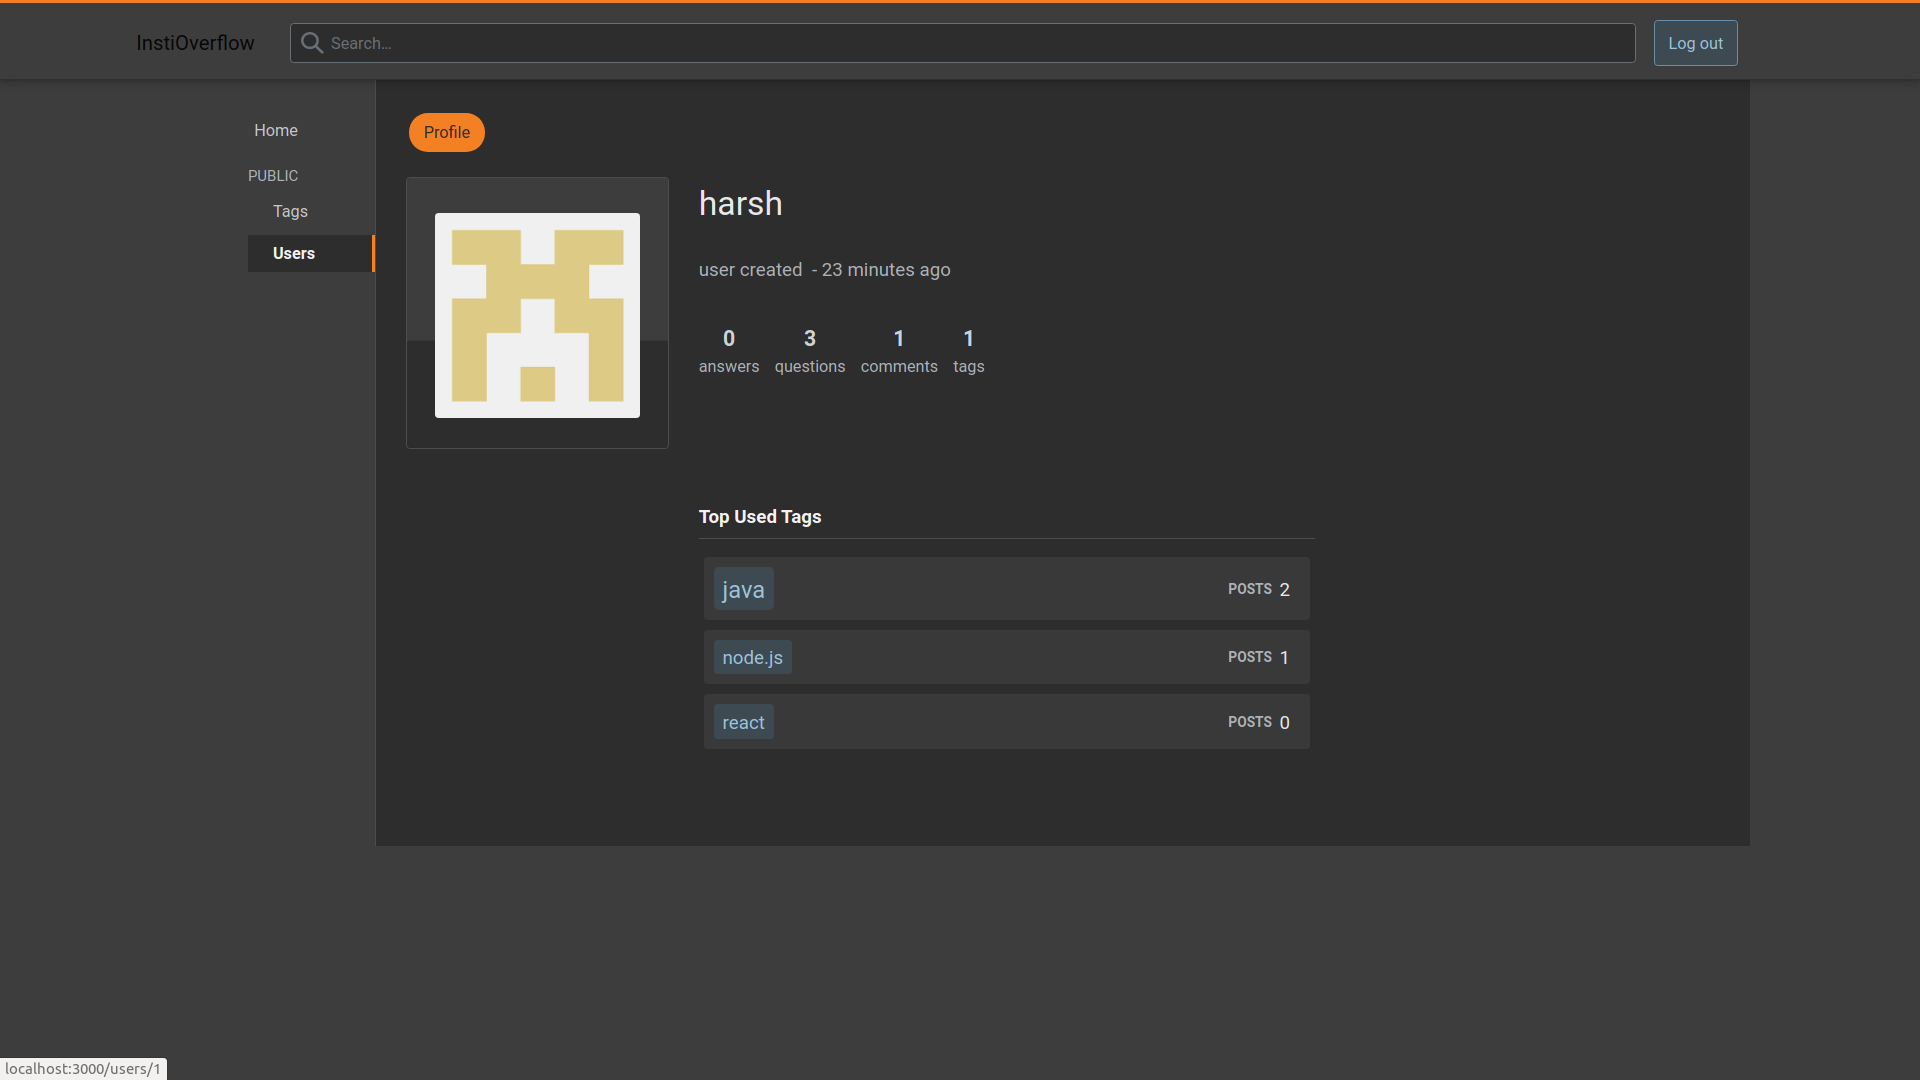
\includegraphics[width=0.75\columnwidth]{User}
\end{center}
\end{figure}



\section{Future Scope}

As of now there is no such global discussion forum for our institute so our project can be extended so that it could be used by the students of our Institute. 



\end{document}
